\section{Instrumentasi Spektrometer Raman}
\label{sec:instrumentasi}

\subsection{Arsitektur Spektrometer Mikro-Raman Konfokal}
Untuk mengkarakterisasi nanomaterial berskala mikrometer seperti serpihan grafena dan berkas nanotube karbon, sistem spektrometer yang digunakan adalah spektrometer mikro-Raman konfokal (\textit{Confocal Micro-Raman Spectrometer}). Arsitektur ini mengintegrasikan mikroskop optik medan-terang dengan spektrograf kisi fokal panjang berresolusi tinggi \cite{smith2019modern}. Diagram blok konfigurasi instrumen disajikan pada Gambar \ref{fig:spectrometer_block}.

\begin{figure}[htbp]
\centering
\resizebox{0.85\textwidth}{!}{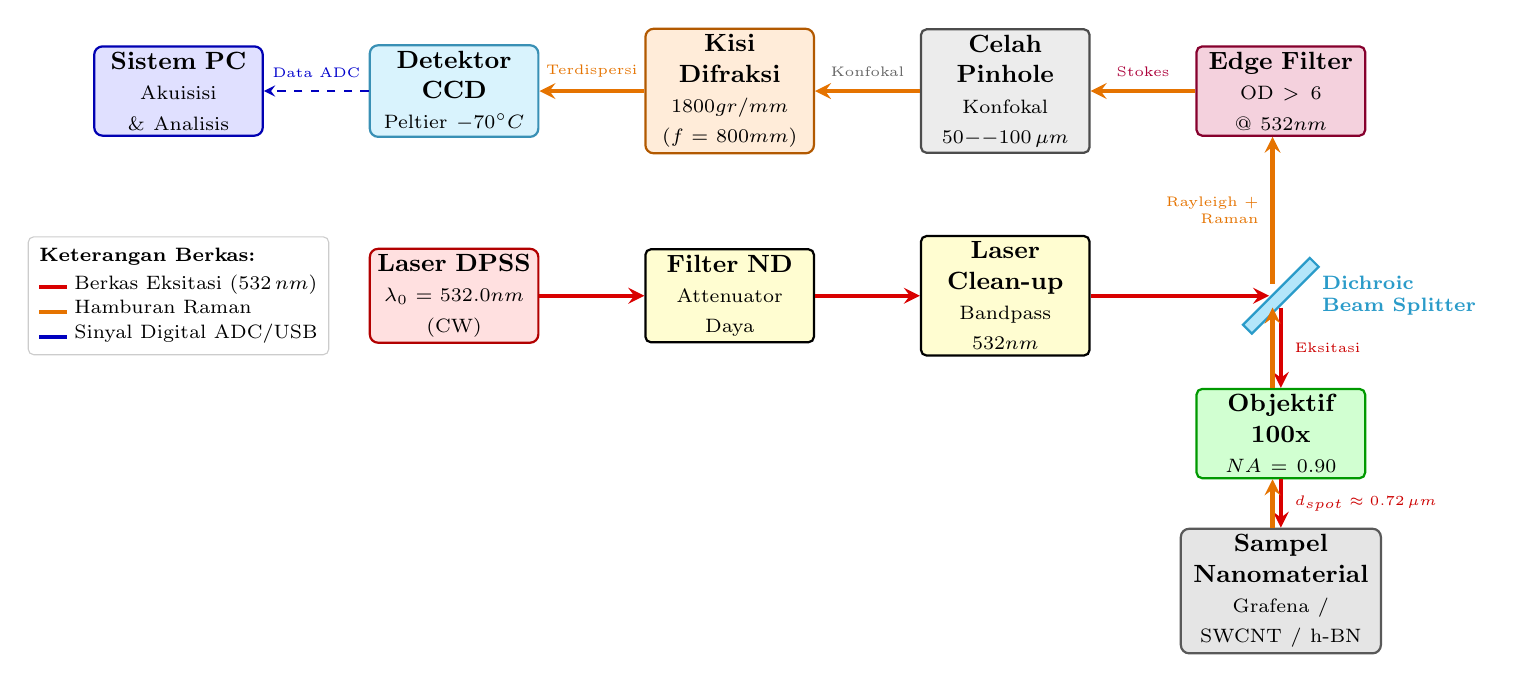
\begin{tikzpicture}[>=stealth, font=\small,
    comp/.style={draw, thick, rounded corners=3pt, align=center, fill=blue!6, text width=2.0cm, minimum height=0.95cm, inner sep=2pt},
    opt/.style={draw, thick, rounded corners=2pt, align=center, fill=yellow!18, text width=2.0cm, minimum height=0.90cm, inner sep=2pt},
    laser_beam/.style={->, line width=1.5pt, red!85!black},
    raman_beam/.style={->, line width=1.5pt, orange!90!black},
    signal_line/.style={->, thick, dashed, blue!75!black}
]
    
    % -------------------------------------------------------------------------
    % BARIS ATAS: DETEKSI & SPEKTROGRAF (y = 2.6)
    % -------------------------------------------------------------------------
    \node[comp, fill=blue!12, draw=blue!70!black] (pc) at (0.0, 2.6) {\textbf{Sistem PC}\\ \scriptsize Akuisisi \& Analisis};
    \node[comp, fill=cyan!15, draw=cyan!70!black] (ccd) at (3.5, 2.6) {\textbf{Detektor CCD}\\ \scriptsize Peltier $-70^\circ\text{C}$};
    \node[comp, fill=orange!15, draw=orange!70!black] (grating) at (7.0, 2.6) {\textbf{Kisi Difraksi}\\ \scriptsize $1800\text{ gr/mm}$ ($f=800\text{ mm}$)};
    \node[opt, fill=gray!15, draw=gray!60!black] (pinhole) at (10.5, 2.6) {\textbf{Celah Pinhole}\\ \scriptsize Konfokal $50\text{--}100\,\mu\text{m}$};
    \node[opt, fill=purple!18, draw=purple!70!black] (edge) at (14.0, 2.6) {\textbf{Edge Filter}\\ \scriptsize OD $>6$ @ $532\text{ nm}$};

    % -------------------------------------------------------------------------
    % BARIS BAWAH: SUMBER EKSITASI & KETERANGAN (y = 0.0)
    % -------------------------------------------------------------------------
    % Legenda di pojok kiri bawah (x = 0.0, y = 0.0)
    \node[draw, rounded corners=2pt, fill=white, draw=gray!40, font=\scriptsize, align=left, inner sep=4pt] (legend) at (0.0, 0.0) {
        \textbf{Keterangan Berkas:}\\[2pt]
        {\color{red!85!black}\rule{0.35cm}{1.4pt}} Berkas Eksitasi ($532\,\text{nm}$)\\[1pt]
        {\color{orange!90!black}\rule{0.35cm}{1.4pt}} Hamburan Raman\\[1pt]
        {\color{blue!75!black}\rule{0.35cm}{1.2pt}} Sinyal Digital ADC/USB
    };

    \node[comp, fill=red!12, draw=red!70!black] (laser) at (3.5, 0.0) {\textbf{Laser DPSS}\\ \scriptsize $\lambda_0 = 532.0\text{ nm}$ (CW)};
    \node[opt] (atten) at (7.0, 0.0) {\textbf{Filter ND}\\ \scriptsize Attenuator Daya};
    \node[opt] (filter_clean) at (10.5, 0.0) {\textbf{Laser Clean-up}\\ \scriptsize Bandpass $532\text{ nm}$};

    % Dichroic Beam Splitter di (14.0, 0.0)
    \draw[thick, draw=cyan!80!black, fill=cyan!30, rotate around={45:(14.0,0.0)}] (13.4,-0.08) rectangle (14.6,0.08);
    \node[right=0.25cm, font=\scriptsize\bfseries, text=cyan!80!black, align=left] at (14.15, 0.0) {Dichroic\\Beam Splitter};

    % -------------------------------------------------------------------------
    % KOLOM VERTIKAL: MIKROSKOP & SAMPEL (x = 14.0, y < 0)
    % -------------------------------------------------------------------------
    \node[opt, fill=green!18, draw=green!60!black] (obj) at (14.0, -1.75) {\textbf{Objektif 100x}\\ \scriptsize $\text{NA} = 0.90$};
    \node[comp, fill=gray!20, draw=gray!70!black, text width=2.4cm] (sample) at (14.0, -3.75) {\textbf{Sampel Nanomaterial}\\ \scriptsize Grafena / SWCNT / h-BN};

    % -------------------------------------------------------------------------
    % JALUR BERKAS EKSITASI (MERAH)
    % -------------------------------------------------------------------------
    \draw[laser_beam] (laser.east) -- (atten.west);
    \draw[laser_beam] (atten.east) -- (filter_clean.west);
    \draw[laser_beam] (filter_clean.east) -- (13.85, 0.0);
    \draw[laser_beam] (14.0, -0.15) -- (obj.north) node[midway, right=1pt, font=\tiny, text=red!80!black] {Eksitasi};
    \draw[laser_beam] (obj.south) -- (sample.north) node[midway, right=1pt, font=\tiny, text=red!80!black] {$d_{\text{spot}} \approx 0.72\,\mu\text{m}$};

    % -------------------------------------------------------------------------
    % JALUR HAMBURAN RAMAN (ORANYE)
    % -------------------------------------------------------------------------
    % Dari sampel kembali ke objektif dan menembus dichroic (digeser sedikit ke kiri)
    \draw[raman_beam] ([xshift=-3pt]sample.north) -- ([xshift=-3pt]obj.south);
    \draw[raman_beam] ([xshift=-3pt]obj.north) -- ([xshift=-3pt]14.0, -0.15);
    \draw[raman_beam] ([xshift=-3pt]14.0, 0.15) -- ([xshift=-3pt]edge.south)
        node[midway, left=1pt, font=\tiny, text=orange!90!black, align=right] {Rayleigh +\\Raman};

    % Jalur dari Edge Filter ke kisi dan detektor
    \draw[raman_beam] (edge.west) -- (pinhole.east) node[midway, above=1pt, font=\tiny, text=purple!90!black] {Stokes};
    \draw[raman_beam] (pinhole.west) -- (grating.east) node[midway, above=1pt, font=\tiny, text=gray!80!black] {Konfokal};
    \draw[raman_beam] (grating.west) -- (ccd.east) node[midway, above=1pt, font=\tiny, text=orange!90!black] {Terdispersi};

    % Sinyal digital dari CCD ke PC
    \draw[signal_line] (ccd.west) -- (pc.east) node[midway, above=1pt, font=\tiny, text=blue!80!black] {Data ADC};

\end{tikzpicture}}
\caption{Diagram blok jalur optik spektrometer mikro-Raman konfokal: penataan berkas eksitasi laser, pemisahan berkas menggunakan \textit{dichroic beam splitter}, pemfokusan mikroskopik 100x pada sampel, penolakan hamburan Rayleigh via \textit{edge filter}, pemilahan spasial konfokal via \textit{pinhole}, dispersi spektral oleh kisi difraksi $1800\text{ gr/mm}$, dan deteksi pada larik CCD berpendingin Peltier $-70^\circ\text{C}$.}
\label{fig:spectrometer_block}
\end{figure}

Jalur berkas optik pada instrumen tersusun atas komponen-komponen kritis berikut:
\begin{enumerate}
    \item \textbf{Sumber Laser Eksitasi}: Laser monokromatik berfase koheren tipe \textit{Diode-Pumped Solid-State} (DPSS) dengan panjang gelombang emisi $\lambda_0 = 532.0\text{ nm}$ ($E_L = 2.3305\text{ eV}$). Berkas dilemahkan menggunakan filter densitas netral (\textit{Neutral Density Filter}, ND) untuk menjaga daya pada permukaan sampel pada rentang aman $0.5 - 2.0\text{ mW}$. Pembatasan daya ini krusial untuk mencegah pemanasan lokal (\textit{laser-induced local heating}) yang dapat menggeser posisi puncak fonon ke frekuensi lebih rendah akibat ekspansi kisi termal.
    \item \textbf{Optik Pengarah dan Pemfokus}: Berkas laser diekspansi dan diarahkan melalui cermin pemisah berkas dikroik (\textit{dichroic beam splitter}) menuju lensa objektif mikroskopik Olympus BX41 berdaya perbesaran 100x dengan bukaan numerik tinggi (\textit{Numerical Aperture}, $\text{NA} = 0.90$). Diameter titik fokus difraksi (\textit{diffraction-limited laser spot size}) dihitung melalui kriteria Airy:
    \begin{equation}
    d_{\mathrm{spot}} \approx \frac{1.22 \lambda_0}{\mathrm{NA}} = \frac{1.22 \times 532\text{ nm}}{0.90} \approx 0.72\text{ }\mu\text{m}.
    \label{eq:spot_size}
    \end{equation}
    Diameter berkas sub-mikrometer ini memungkinkan analisis spasial lokal pada batas butir, tepi defek, atau area transfer heterostruktur secara presisi.
    \item \textbf{Geometri Pengumpulan Hamburan}: Pengumpulan sinyal hamburan dilakukan dalam geometri hamburan balik $180^\circ$ (\textit{backscattering geometry}, $\mathbf{k}_s \approx -\mathbf{k}_0$) menggunakan lensa objektif mikroskop yang sama, memaksimalkan efisiensi penangkapan foton terhambur.
    \item \textbf{Filter Penolak Hamburan Elastik Rayleigh}: Sinyal yang dikumpulkan terdiri atas hamburan elastik Rayleigh yang sangat kuat dan sinyal hamburan inelastik Raman yang lemah (rasio intensitas $\sim 10^{-6} - 10^{-8}$). Untuk mencegah saturasi detektor CCD dan pancaran cahaya sesatan (\textit{stray light}), digunakan \textit{dielectric edge filter} bertingkat tinggi dengan kerapatan optik (\textit{Optical Density}) $\text{OD} > 6$ pada $532\text{ nm}$. Filter ini menolak garis laser Rayleigh hingga faktor $10^6$ dan meloloskan foton Stokes dengan tepi cut-off tajam pada $\approx 50\text{ cm}^{-1}$.
    \item \textbf{Celah Konfokal (\textit{Confocal Pinhole})}: Aperture celah konfokal berdiameter $50 - 100\text{ }\mu\text{m}$ diletakkan pada bidang fokal konjugat detektor. Pinhole ini memblokir berkas cahaya di luar bidang fokus (\textit{out-of-focus light}), menghasilkan resolusi kedalaman aksial tinggi ($\Delta z \le 1.5\text{ }\mu\text{m}$) yang mengeliminasi sinyal latar belakang luminesensi dari substrat tebal.
    \item \textbf{Spektrograf Czerny--Turner dan Kisi Difraksi}: Berkas Raman difokuskan ke celah masuk spektrograf Czerny--Turner fokal panjang ($f = 800\text{ mm}$), dipantulkan oleh cermin kolimator menuju kisi difraksi refleksi holografik bertakik $1800\text{ grooves/mm}$.
    \item \textbf{Detektor Larik CCD}: Spektrum yang terdispersi diproyeksikan ke sensor kamera \textit{Charge-Coupled Device} (CCD) Synapse dengan format matriks $1024 \times 256$ piksel. Sensor didinginkan secara termoelektrik (Peltier) hingga temperatur $-70^\circ\text{C}$ untuk menekan arus gelap hingga $< 0.002\text{ e}^-/\text{piksel/detik}$.
\end{enumerate}

\subsection{Persamaan Kisi Difraksi dan Resolusi Spektral}
Dispersi spasial foton hamburan terhadap panjang gelombang diatur oleh persamaan difraksi kisi:
\begin{equation}
m \lambda = d (\sin \theta_i + \sin \theta_d),
\label{eq:persamaan_kisi}
\end{equation}
dengan $m$ menyatakan orde difraksi ($m = 1$ untuk moda standar), $d = 10^6 / 1800 \approx 555.56\text{ nm}$ adalah jarak antar-alur kisi, $\theta_i$ adalah sudut datang berkas terhadap garis normal kisi, dan $\theta_d$ adalah sudut difraksi berkas terhambur.

Dispersi sudut kisi difraksi diberikan oleh turunan sudut difraksi terhadap panjang gelombang:
\begin{equation}
D_{\theta} = \frac{d\theta_d}{d\lambda} = \frac{m}{d \cos \theta_d}.
\label{eq:dispersi_sudut}
\end{equation}

Dispersi linier pada bidang fokal detektor CCD dengan panjang fokal spektrograf $f = 800\text{ mm}$ bernilai:
\begin{equation}
\frac{dx}{d\lambda} = f \frac{d\theta_d}{d\lambda} = \frac{f \cdot m}{d \cos \theta_d}.
\label{eq:dispersi_linier}
\end{equation}

Untuk detektor dengan lebar fisik piksel $w_{\mathrm{pix}} = 26\text{ }\mu\text{m}$, dispersi timbal-balik per piksel pada daerah spektrum $\lambda \approx 580\text{ nm}$ ($\Delta\tilde{\nu} \approx 1580\text{ cm}^{-1}$) adalah:
\begin{equation}
\delta\lambda_{\mathrm{pix}} = \frac{w_{\mathrm{pix}}}{dx/d\lambda} \approx 0.016\text{ nm/pixel}.
\end{equation}

Dinyatakan dalam bilangan gelombang, resolusi pergeseran Raman per piksel diberikan oleh diferensiasi $\Delta\tilde{\nu} = 10^7 (1/\lambda_0 - 1/\lambda_s)$:
\begin{equation}
\delta\tilde{\nu} = \frac{10^7}{\lambda_s^2} \delta\lambda \approx \frac{10^7}{(580\text{ nm})^2} (0.016\text{ nm}) \approx 0.47\text{ cm}^{-1}/\text{pixel}.
\label{eq:resolusi_spektral}
\end{equation}
Resolusi instrumen $\le 0.5\text{ cm}^{-1}$ ini sangat memadai untuk memisahkan dekonvolusi komponen sub-pita yang memiliki selisih pergeseran beberapa $\text{cm}^{-1}$.

\subsection{Kalibrasi Bilangan Gelombang dan Verifikasi Stabilitas}
Akurasi posisi bilangan gelombang dijamin melalui kalibrasi standar menggunakan fonon optik kisi kristal tunggal Silikon monokristalin $\text{Si}(100)$ pada orientasi normal. Mode fonon optik $F_{2g}$ silikon memiliki frekuensi acuan internasional yang terstandarisasi:
\begin{equation}
\Delta\tilde{\nu}_{\mathrm{Si}} = 520.70 \pm 0.05\text{ cm}^{-1}.
\label{eq:kalibrasi_silikon}
\end{equation}
Penyimpangan posisi puncak silikon dikoreksi melalui kalibrasi offset motorik kisi monokromator sebelum pengambilan data spektral, menjamin akurasi absolut pergeseran Raman lebih baik dari $\pm 0.2\text{ cm}^{-1}$.
